\documentclass[a4paper]{report}
\usepackage[utf8]{inputenc}
\usepackage{amsmath}
\usepackage{esint}
\usepackage{tabstackengine}
\usepackage[colorlinks,linkcolor=blue]{hyperref}
\usepackage{xeCJK}
%\usepackage{ctex}
\usepackage{caption} 
%\usepackage{minted}
\usepackage{stackengine}
\usepackage{graphicx}
\graphicspath{ {../resources/figure/poss/} }
\usepackage{float}
\usepackage{amsmath}
\usepackage{ulem}
\usepackage{amssymb}
\usepackage{tabularx}
\usepackage{multirow}
\usepackage{tikz}
\usetikzlibrary{calc}
\usetikzlibrary{shapes,arrows}
\usepackage{pgfplots}
\usepackage{diagbox}
%%%% 下面的命令重定义页面边距,使其符合中文刊物习惯 %%%%
\addtolength{\topmargin}{-54pt}
\setlength{\oddsidemargin}{0.63cm}  % 3.17cm - 1 inch
\setlength{\evensidemargin}{\oddsidemargin}
\setlength{\textwidth}{14.66cm}
\setlength{\textheight}{24.00cm}    % 24.62

%%%% 段落首行缩进两个字 %%%%
% \makeatletter
% \let\@afterindentfalse\@afterindenttrue
% \@afterindenttrue
% \makeatother
% \setlength{\parindent}{2em}  %中文缩进两个汉字位

% 段首不缩进
\setlength{\parindent}{0pt}
%%%% 下面的命令设置行间距与段落间距 %%%%
\linespread{1.4}
% \setlength{\parskip}{1ex}
\setlength{\parskip}{0.5\baselineskip}

\newcommand{\tabincell}[2]{\begin{tabular}{@{}#1@{}}#2\end{tabular}}
\captionsetup[table]{skip=10pt}

\title{Possibility Note}
\author{Crosstyan}
\date{Augest 2020}
\begin{document}
\chapter{Introduction}
\section{Sample Space}
\begin{itemize}
  \item 相同条件
  \item 实验结果不止一个(可以事先确定所有的可能结果)
  \item 进行一次实验之前不确定结果
\end{itemize}
样本空间的子集为事件. 样本空间的元素为样本点. $S$(样本空间)必然发生, 为必然事件. $\varnothing$(空集)不包含任何样本点, 为不可能事件. 
\section{公式}
\subsection{加法}
$$P(A\cup B)=P(A)+P(B)-P(A\cdot B)=P(A\cdot\bar{B})+P(\bar{A}\cdot B)+P(A\cdot B)$$
\subsection{减法}
$$P(A-B)=P(A\bar{B})=P(A)-P(A\cdot B)$$
\subsection{乘法}
若$P(A) > 0$, 则
\begin{align*}
  P(A\cap B)&=P(A\cdot B)\\
  &=P(B\mid A) \cdot P(A)\\
  &=P(A\mid B)\cdot P(B)
\end{align*}
必须考虑A和B是否独立, 若不独立不可以概率直接相乘得到积概率. 
\subsection{取反}
\begin{align*}
  P(\bar{A})&=1-P(A)\\
  P(\overline{AB})&=1-P(AB)
\end{align*}
\subsection{全概率}
设有一样本空间$S$, 其中$A$为随机事件$B_1,B_2,B_3\dots B_n$的划分, 且$P(B_i)>0$, 则
$$P(A)=\sum_{i=1}^n P(A\mid B_i)\cdot P(B_i)$$
划分$\mathbb{B}$并起来等于$S$, 且两两互不相交. 
\subsection{贝叶斯}
$$P(B_j\mid A)=\frac{P(A\mid B_j)\cdot P(B_j)}{\sum_{i=1}^n P(A\mid B_i)\cdot P(B_i)}$$
\section{条件概率}
条件概率本质就是压缩样本空间
\begin{align*}
  P(B\mid A)&=\frac{P(AB)}{P(A)}\\
  &=\frac{P(A\mid B)\cdot P(B)}{P(A)}\\
  P(A\mid B)&=\frac{P(AB)}{P(B)}\\
  &=\frac{P(B\mid A)\cdot P(A)}{P(B)}
\end{align*}
设$S$为样本空间
\begin{align*}
  P(B)&=\frac{P(B\cdot S)}{P(S)}\\
  P(S)&=1
\end{align*}
\section{完备事件组}
若事件$B_1,B_2,B_3\dots B_n$两两互斥, 且$B_1\cup B_2\cup B_3\dots \cup B_n=S$($S$为样本空间), 则称$B_1,B_2,B_3\dots B_n$为一个完备事件组. 
\section{独立事件}
若事件$A, B$相互独立, 则. 
$$\begin{cases}
  P(A\mid B)=P(A)\\
  P(B\mid A)=P(B)
\end{cases}
$$
$$P(A\cdot B)=P(A)\cdot P(B)$$
\section{应用题}
\begin{enumerate}
  \item 甲乙独立对同一目标射击一次, 命中率分别为0.6和0.5, 求两人中至少一人射中的概率. 
  \item 从甲乙任选一人同一目标射击一次, 命中率分别为0.6和0.5, 求目标被射中的概率. 
  \item 甲乙独立对同一目标射击一次, 命中率分别为0.6和0.5, 已知目标命中, 求是甲射中的概率. 
  \item 从甲乙任选一人同一目标射击一次, 命中率分别为0.6和0.5, 已知目标命中, 求是甲射中的概率. 
\end{enumerate}
\section{总结}
\begin{itemize}
  \item 积事件的概率和条件概率
  \item 独立的积事件和不独立的
  \item 正面做和反面做 (至多, 至少)
  \item 样本空间的划分
\end{itemize}
重点
\begin{itemize}
  \item 随机事件的概念
  \item 古典概型的概率计算方法
  \item 概率的加法公式
  \item 条件概率和乘法公式的应用
  \item 全概率公式和贝叶斯公式的应用
\end{itemize}
\chapter{一维随机变量}

\section{Possibility Distribution Functions}
\subsection{PDF}
Possibility Density Function. 概率密度函数. 
$$f(x)\geq 0$$
被称为非负性
$$\int_{-\infty}^{+\infty}f(x)\;dx=1$$
被称为归一性\\
$$P \{a<X\leq b\}=\int_a^b f(x)\;dx$$
哪里求变量哪里求积分
\subsection{PMF}
Possibility Mass Function. 又被称为分布率. \\
离散型的PDF
\subsection{CDF}
Cumulative Distribution Function. 累积分布函数. 
$$F(x)=P\{X\leq x\}$$
\begin{align*}
F(-\infty)&=0\\
F(+\infty)&=1
\end{align*}
CDF单调递增 (累积, 不会减少)\\
\begin{align*}
  P\{X=k\}&=P\{X\leq k\}-P\{X<k\}\\
  &=F(k)|_{x\geq k\text{的那部分函数}}-F(k)|_{x<k\text{的那部分函数}}
\end{align*}
若$k$在边界. 
\subsection{PDF到CDF}
若有PDF
\begin{align*}
  f(x)=\begin{cases}
    f_1(x),&a\leq x<b\\
    f_2(x),&b\leq x<c\\
    f_3(x),&c\leq x<d\\
    0,&\text{elsewhere.}
  \end{cases}\\
\end{align*}
则有CDF
\begin{align*}
  F(x)=\begin{cases}
    0,&x<a\\
    \int_a^x f_1(x)\;dx,&a\leq x<b\\
    \int_a^b f_1(x)\;dx+\int_b^x f_2(x)\;dx,&b\leq x<c\\
    \int_a^b f_1(x)\;dx+\int_b^c f_2(x)\;dx+\int_c^x f_3(x)\;dx,&c\leq x<d\\
    1,&x>c
  \end{cases}
\end{align*}
\section{连续性随机变量的函数}
若$Y=g(X)$
\section{$Y=g(X)$单调可导}
\begin{itemize}
  \item 求$Y=g(X)$的值域
  \item $Y=g(X)\Rightarrow$关于$X$的函数(反函数) $x=h(y)$
  \item $f_Y(y)=f_X[h(y)]\cdot |\frac{d h(y) }{d y}|$
\end{itemize}
\section{$Y=g(X)$非单调可导}
\begin{figure}[H]
\centering
\begin{tikzpicture}
  \node (fx){$f_X(x)$};
  \node[right of =fx, node distance=4cm] (FY){$F_Y(y)$};
  \node[right of = FY, node distance=2cm] (fy){$f_Y(y)$};
  
  \path[draw, -latex'] (fx)--node[above]{\color{red} find $P\{g(X)\leq y\}$} (FY);
  \path[draw, -latex'] (FY)--node[above]{\color{red}  $\frac{d}{dy}$} (fy);
  \end{tikzpicture}
\caption{步骤图}
\end{figure}
先求$Y$的CDF ($F_Y$) 然后求导得到$f_Y$\\
还是得求$Y=g(X)$的值域
\begin{align*}
  F_Y(y)&=P\{Y\leq y\}\\
  &=P\{g(X)\leq y\}\\
  &=P \{X\leq h(y)\}&& \text{$h(y)$为$g(X)$的反函数}\\
  &=F_X[h(y)]\\
  f_Y(y)&=F_Y'(y)\\
  &=\frac{d  }{d \,[h(y)]} F_X[h(y)] \cdot \frac{d\,[h(y)]}{d y}\\
  &=f_X[h(y)]\cdot \frac{d\,[h(y)]}{d y}
\end{align*}

\paragraph{例子}下面是很麻烦的例子, 不用看了. 直接套用上面的方法就好了, 没必要分类讨论. 
\begin{align*}
  f_X(x)=\begin{cases}
    2x,&0<x\leq 1\\
    0, &\text{elsewhere}
  \end{cases}
\end{align*}
求$Y=e^{-X}$的PDF.
\subparagraph{假解}根据$P \{a<X\leq b\}=\int_b^a f(x)\;dx=F(b)-F(a)$易知
\begin{align*}
  F_Y(y)&=P \{Y\leq y\}\\
  &=P \{e^{-X}\leq y\} 
\end{align*}
开始分类讨论\\
$y\leq 0$时, $P \{e^{-X}\leq y\}=0$ (因为$e^{-X}$值域大于0)\\
$y>0$时, $P \{e^{-X}\leq y\}=P \{X\geq -\ln(y)\}$\\
就可以转换为$P \{X\leq b\}=\int_b^{+\infty} f(x)\;dx$的情况. \\
积分区间就为$[-\ln(y),+\infty)$与$(0,1)$的交集. \\
所以可以根据$(0,1)$确定$-\ln(y)$的取值. 
\subparagraph{真解} 易得
\begin{align*}
  F_Y(y)&=P\{Y\leq y\}\\
  &=P\{ e^{-X}\leq y\}\\
  &=P \{X\leq -\ln(y)\}\\
  &=F_X[-\ln(y)]\\
  f_Y(y)&=F_Y'(y)\\
  &=\frac{d  }{d \,[-\ln(y)]} F_X[-\ln(y)] \cdot \frac{d\,[-\ln(y)]}{d y}\\
  &=f_X[-\ln(y)]\cdot \frac{d\,[-\ln(y)]}{d y}\\
  &=2\cdot(-\ln y)\cdot \frac{-1}{y}\\
  &=\frac{2\ln y}{y}
\end{align*}
与正确答案差一个负号, 可能是因为定义域映射到值域反转了一下? 

\chapter{二维随机变量}
% Table generated by Excel2LaTeX from sheet 'Sheet1'
\begin{table}[H]
  \centering
  \caption{联合分布和边缘分布的例子}
    \begin{tabular}{c|ccc|c}
    \diagbox{$X$}{$P$}{$Y$}    & 100   & 90    & 70    & $X_\text{marginal}$ \\
    \hline
    100   & 0.01  & 0.02  & 0.07  & 0.1 \\
    80    & 0.02  & 0.04  & 0.14  & 0.2 \\
    40    & 0.07  & 0.14  & 0.49  & 0.7 \\
    \hline
    $Y_\text{marginal}$     & 0.1   & 0.2   & 0.7   & 1 \\
    \end{tabular}%
\end{table}%
其中$P$代表$P \{X=i,Y=j\}$的概率 (联合分布). \\
$X_\text{marginal}=P \{X=x_i\}$, $Y_\text{marginal}=P \{Y=y_j\}$
\section{Union Distribution}
\subsubsection{离散型}
% Table generated by Excel2LaTeX from sheet 'Sheet1'
\begin{table}[htbp]
  \centering
  \caption{联合分布}
    \begin{tabular}{c|ccc}
    \diagbox{$X$}{$P$}{$Y$}    & 100   & 90    & 70 \\
    \hline
    100   & 0.01  & 0.02  & 0.07 \\
    80    & 0.02  & 0.04  & 0.14 \\
    40    & 0.07  & 0.14  & 0.49 \\
    \end{tabular}%
\end{table}%
其中$P$代表$P \{X=i,Y=j\}$的概率 (联合分布). 
\subsubsection{连续型}
$$f(x,y)$$
有着类似的非负性和归一性. 
\begin{align*}
  f(x,y)&\geq 0\\
  \int_{-\infty}^{+\infty}dx\int_{-\infty}^{+\infty} f(x,y) \;dy&=1
\end{align*}

哪里求概率哪里求积分
\begin{align*}
  P \{(X,Y)\in D \}=\iint_D f(x,y)\;dx\;dy
\end{align*}
\subsubsection{CDF}
$$F(x,y)=P \{X\leq x,\,Y\leq y\}$$

\section{Marginal Distribution}
\subsubsection{离散型}
\begin{align*}
  P \{X=x_i\}=\sum_{i=1}^\infty P \{X=x_i,\,Y=y_j\}
\end{align*}

可以列出$X$和$Y$的边缘PMF, 以$P \{X=100\}$为例. 
\begin{align*}
  &P \{X=100\}\\
  &=P \{X=100,Y=100\}+P \{X=100,Y=90\}+P \{X=100,Y=70\}\\
\end{align*}
% Table generated by Excel2LaTeX from sheet 'Sheet1'
\begin{table}[htbp]
  \centering
  \caption{$X$的边缘分布}
    \begin{tabular}{c|ccc}
    $X$     & 100   & 80    & 40 \\
    \hline
    $P \{X=x_i\}$     & 0.1   & 0.2   & 0.7 \\
    \end{tabular}%
\end{table}%

% Table generated by Excel2LaTeX from sheet 'Sheet1'
\begin{table}[htbp]
  \centering
  \caption{$Y$的边缘分布}
    \begin{tabular}{c|ccc}
    $Y$     & 100   & 90    & 70 \\
    \hline
    $P \{Y=y_j\}$     & 0.1   & 0.2   & 0.7 \\
    \end{tabular}%
\end{table}%

\subsubsection{连续型}
通过对$y$的积分来求$X$的概率密度, 竖着切\\
通过对$x$的积分来求$Y$的概率密度, 横着切
\begin{align*}
  f_X(x)&= \int_{-\infty}^{+\infty} f(x,y)\; dy&&\text{最后的结果只有$x$, 积分上下限关于$x$}\\
  f_Y(y)&= \int_{-\infty}^{+\infty} f(x,y)\; dx&&\text{最后的结果只有$y$, 积分上下限关于$y$}
\end{align*}

\subsubsection{CDF}
\begin{align*}
  F_X(x)&=\lim_{x\rightarrow +\infty} F(x,y)\\
  F_Y(y)&=\lim_{y\rightarrow +\infty} F(x,y)
\end{align*}
\section{Conditional Distribution}
条件概率联合分布比边缘分布. 
$$\text{条件}=\frac{\text{联合}}{\text{边缘}}$$
\begin{align*}
  f_{X|Y}(x|y)&=\frac{f(x,y)}{f_Y(y)}&&\text{是一个关于$x$的函数 (不含有y) $f_Y(y)\neq 0$}
\end{align*}
\section{连续型随机变量的函数的概率分布}
\subsection{$Z=X+Y$}

谁在函数中的表达式较为简单就换谁(在此以$Y=Z-X$为例)
$$f_z(z)=\int_{-\infty}^{+\infty}f(x,z-x)\;dx$$
积分上下限必定有$z$\\
相当于求关于$z$的\textbf{边缘概率密度}, 故不用求CDF. \\
关键是确定$x$(被积变量) 的积分区域. 
根据题目的变量不等式来列出被积变量的不等式, 一般会有
\begin{itemize}
  \item 中间是被积变量$x$, 两边为关于$z$的不等式. 
  \item 中间是被积变量$x$, 两边为常数 (或者只有单边)的不等式
  \item 其他限制条件 (不等式)
\end{itemize}
\begin{align*}
  \begin{cases}
    a<x<b\\
    z-a<x<z+b
  \end{cases}
\end{align*}
取$z$关于被积变量的交集, 可以得到$z$的范围. 
\begin{figure}[h]
  \centering
  % \begin{tikzpicture}
  %   \draw [->] (-5,0)--(5,0);
  %   \draw [color=red](1,0)--(1,.5)--(3,.5)--(3,0);
  %   \draw (0,0)--(0,.7)--(5,.7);
  %   \fill [color=red!30](1,0) rectangle (3,.5);
  %   \node[fill=white,draw=black,circle,inner sep=2pt,label=below:{$z-1$}] at (1,0){};
  %   \node[fill=white,draw=black,circle,inner sep=2pt,label=below:{$z$}] at (3,0){};
  %   \node[fill=white,draw=black,circle,inner sep=2pt,label=below:{$0$}] at (0,0){};
  % \end{tikzpicture}

  %\usetikzlibrary{calc}
  %for calculation coords
  \begin{tikzpicture}
    \coordinate (Start) at (-5,0);
    \coordinate (End) at (5,0);
    \coordinate (A) at (1,0);
    \coordinate (B) at (3,0);
    \coordinate (Height1) at (0,0.7);
    \coordinate (Height2) at (0,.5);
    \coordinate (C) at (0,0);
    \draw [->] (Start)--(End);
    \draw [color=red](A)--++(Height2)--($(B)+(Height2)$)--(B);
    \draw (C)--($(C)+(Height1)$)--($(End)+(Height1)$);
    %\fill [color=red!30](1,0) rectangle (3,.5);
    \node[fill=white,draw=black,circle,inner sep=2pt,label=below:{$z-1$}] at (A){};
    \node[fill=white,draw=black,circle,inner sep=2pt,label=below:{$z$}] at (B){};
    \node[fill=white,draw=black,circle,inner sep=2pt,label=below:{$0$}] at (C){};
  \end{tikzpicture}
  \begin{tikzpicture}
    \coordinate (Start) at (-5,0);
    \coordinate (End) at (5,0);
    \coordinate (A) at (-1,0);
    \coordinate (B) at (1,0);
    \coordinate (Height1) at (0,0.7);
    \coordinate (Height2) at (0,.5);
    \coordinate (C) at (0,0);
    \draw [->] (Start)--(End);
    \draw [color=red](A)--++(Height2)--($(B)+(Height2)$)--(B);
    \draw (C)--($(C)+(Height1)$)--($(End)+(Height1)$);
    %\fill [color=red!30](1,0) rectangle (3,.5);
    \node[fill=white,draw=black,circle,inner sep=2pt,label=below:{$z-1$}] at (A){};
    \node[fill=white,draw=black,circle,inner sep=2pt,label=below:{$z$}] at (B){};
    \node[fill=white,draw=black,circle,inner sep=2pt,label=below:{$0$}] at (C){};
  \end{tikzpicture}
  \begin{tikzpicture}
    \coordinate (Start) at (-5,0);
    \coordinate (End) at (5,0);
    \coordinate (A) at (-3,0);
    \coordinate (B) at ($(A)+(2,0)$);
    \coordinate (Height1) at (0,0.7);
    \coordinate (Height2) at (0,.5);
    \coordinate (C) at (0,0);
    \draw [->] (Start)--(End);
    \draw [color=red](A)--++(Height2)--($(B)+(Height2)$)--(B);
    \draw (C)--($(C)+(Height1)$)--($(End)+(Height1)$);
    %\fill [color=red!30](1,0) rectangle (3,.5);
    \node[fill=white,draw=black,circle,inner sep=2pt,label=below:{$z-1$}] at (A){};
    \node[fill=white,draw=black,circle,inner sep=2pt,label=below:{$z$}] at (B){};
    \node[fill=white,draw=black,circle,inner sep=2pt,label=below:{$0$}] at (C){};
  \end{tikzpicture}
  \caption{}
\end{figure}

\subsection{$Z=XY$}
\begin{align*}
  Z&=XY\\
  X&=\frac{Z}{Y}\\
  Y&=\frac{Z}{X}
\end{align*}
\begin{align*}
  f_Z(z)=\int_{-\infty}^{+\infty} \frac{1}{|x|}\cdot f(x,\frac{z}{x})\;dx
\end{align*}
积分上下限必定有$z$\\
注意前边有个$\frac{1}{|x|}$. \\
不等式形式为: $x$在中间一个, $z$在中间一个. 

\begin{align*}
  \begin{cases}
    a<x<b\\
    a<z<x
  \end{cases}
\end{align*}
\subsection{$Z=max \{X,Y\}$}
\begin{itemize}
  \item 先求边缘CDF $F_X,F_Y$
  \item $F_{\text{max}}=F_X(z)\cdot F_Y(z)$
  \item $F_{\text{min}}(z)=1-[1-F_X(z)]\cdot[1-F_Y(z)]$  取边缘CDF与1差值之积, 再取积与1差值
  \item $f_\text{max}(z)=\frac{d F_{\text{max}}(z) }{d z}$
\end{itemize}
若$X,Y$独立同分布
\begin{itemize}
  \item $F_{\text{max}}=[F_X(z)]^2$
  \item $f_{\text{max}}=F_{\text{max}}'(z)$
\end{itemize}
若有$n$个随机变量相互独立且具有相同分布$F(x)$. 
\begin{align*}
  F_{\text{max}}&=[F(z)]^n &&z=\text{max}(X_1,X_2,X_3\dots ,X_n)\text{的分布函数}\\
  F_{\text{min}}&=1-[1-F(z)]^n &&z=\text{min}(X_1,X_2,X_3\dots ,X_n)\text{的分布函数}
\end{align*}
\section{两个随机变量的独立性}
联合等于两个边缘相乘则独立. 
\begin{align*}
  f(x,y)=f_X(x)\cdot f_Y(y) &\Longleftrightarrow \text{$X$与$Y$独立 (充要条件)}\\
  f_{X\mid Y}(x\mid y)=f_X(x)&\Longleftrightarrow \text{$X$与$Y$独立}
\end{align*}
\subsection{求分布律未知量}
\textbf{若$X,Y$相互独立}\\
先列出边缘分布. 联合分布率等于边缘分布率相乘 (可以任意列). \\
也可以用归一性, ($X$和$Y$的) 边缘分布之和为1. \\
当然最好算的是\textbf{各行各列成比例}. \\
\subsection{连续型的独立性}
若$X,Y$相互独立, 则其联合概率密度(PDF)中函数值非零的区域必为方形区域$a<x<b,\, c<y<b$. (必要不充分)

\section{补充: 二重积分}
\subsection{竖着切}
\begin{figure}[H]
\centering
\includegraphics[width=0.33\textwidth]{cut_x.png}
\caption{竖着切 (X型区域)}
\end{figure}
往哪切哪边就是常数, 提出来放到左边. \\
画两条竖线$x=a,\,x=b$, 作为边缘, 当然是常数. \\
上下是关于$x$的函数 $y=g_1(x),\,y=g_2(x)$, RHS不含$y$, LHS就是$y$. \\
从左到右, 从下到上.
$$\int_a^b dx\int_{g_1(x)}^{g_2(x)}f(x,y)\;dy$$
$$\int_a^b [\int_{g_1(x)}^{g_2(x)}f(x,y)\;dy]\;dx$$
\subsection{横着切}
\begin{figure}[H]
\centering
\includegraphics[width=0.33\textwidth]{cut_y.png}
\caption{横着切 (Y型区域)}
\end{figure}
往哪切哪边就是常数, 提出来放到左边. \\
画两条横线$y=a,\,y=b$, 作为边缘, 当然是常数. \\
上下是关于$y$的函数 $x=h_1(y),\,x=h_2(y)$, RHS不含$x$, LHS就是$x$. \\
从下到上, 从左到右. 
$$\int_a^b dy\int_{h_1(y)}^{h_2(y)}f(x,y)\;dx$$
\chapter{随机变量的数字特征}
\section{常见分布}
\subsection{二项分布}
$X\sim\mathcal{B}\;(n,p)$
$$P \{X=k\}=\binom{n}{k}\cdot p^{k}\cdot (1-p)^{n-k}$$
$E(X)=np\\D(X)=n p\cdot (1-p)$
\subsubsection{两点分布}
又被称作0--1分布, 就是$X\sim \mathcal{B}\;(1,p)$的情况
$$P \{X=k\}=p^k\cdot (1-p)^{1-k}=
\begin{cases}
  p&k=1,\\
  (1-p)&k=0.
\end{cases}$$
\subsection{泊松分布}
$X\sim \pi(\lambda)$
$$P\{x=k\}=\frac{\lambda^k \cdot e^{-\lambda}}{k\;!}$$
$E(X)=\lambda \\ D(X)=\lambda$
\subsection{正态分布}
$X\sim \mathcal{N}(\mu,\sigma^2)$
$$f(x)=\frac{1}{\sqrt{2\pi}\cdot \sigma}\cdot e^{-\frac{(x-\mu)^2}{2\cdot\sigma^2}}$$
$E(X)=\mu \\ D(X)=\sigma^2$
\subsubsection{标准正态分布}
服从$\mu=0,\;\sigma=1$的正态分布\\
若$X\sim \mathcal{N}(\mu,\sigma^2)$
$$Z=\frac{X-\mu}{\sigma}\sim \mathcal{N}(0,1)$$
\paragraph{性质}标准正态分布具有如下性质
\begin{itemize}
  \item $\mu=0$, $\Phi(0)=\frac{1}{2}$
  \item $\Phi(-x)=1-\Phi(x)$
\end{itemize}
若$X\sim \mathcal{N}(\mu,\sigma^2)$
\begin{itemize}
  \item $\frac{X-\mu}{\sigma}\sim \mathcal{N}(0,1)$
  \item $P \{X<a\}=\Phi(\frac{a-\mu}{\sigma})$
  \item $P \{a<X<b\}=\Phi(\frac{b-\mu}{\sigma})-\Phi(\frac{a-\mu}{\sigma})$
\end{itemize}
\subsubsection{正态分布的线性组合}
若$X\sim \mathcal{N}(\mu_1,\sigma_1^2)$ $Y\sim \mathcal{N}(\mu_2,\sigma_2^2)$且$X$与$Y$相互独立则
$$X\pm Y\sim \mathcal{N}(\mu_1\pm \mu_2,\sigma_1^2+\sigma_2^2)$$
\par 若$U\sim \mathcal{N}(\mu,\sigma^2)$, $V=aU+b$
$$V\sim \mathcal{N} (a\mu+b,a^2\sigma^2)$$
\subsection{指数分布}
$$f(x)=\begin{cases}
  \frac{1}{\lambda}\cdot e^{-\frac{1}{\lambda}\cdot x}&x>0,\\
  0&\text{elsewhere.}
\end{cases}$$
$E(X)=\lambda \\ D(X)=\lambda^2$
\subsection{均匀分布}
$$f(x)=\begin{cases}
  \frac{1}{b-a}&a<x<b,\\
  0&\text{elsewhere.}
\end{cases}$$
$E(X)=\frac{a+b}{2}\\D(X)=\frac{(b-a)^2}{12}$
\section{期望值}
本质为加权平均. 
$$E(X)=\sum_{i=1}^{+\infty}X_i\cdot P \{X=X_i\} $$
$$E(x)=\int_{-\infty}^{+\infty}x\cdot f(x)\;dx$$
参数为一维函数情况. 
\begin{align*}
  E[g(x)]&=\sum_{i=1}^{+\infty}g(x_i)\cdot P \{X=x_i\}\\
  E[g(x)]&=\int_{-\infty}^{+\infty}g(x)\cdot f(x)\;dx\\
  E(x^2)&=\int_{-\infty}^{+\infty}x^2\cdot f(x)\;dx &&\text{注意$f(x)$的参数仍然是$x$}
\end{align*}
参数为二维函数情况 (积事件, 联合分布率)
\begin{align*}
  E(x)&=\int_{-\infty}^{+\infty}\;dx\int_{-\infty}^{+\infty}x\cdot f(x,y)\;dy\\
  E(y)&=\int_{-\infty}^{+\infty}\;dx\int_{-\infty}^{+\infty}y\cdot f(x,y)\;dy\\
  E[g(x,y)]&=\int_{-\infty}^{+\infty}\;dx\int_{-\infty}^{+\infty}g(x,y)\cdot f(x,y)\;dy\\
\end{align*}

\section{方差}
平方的期望减去期望的平方
$$D(X)=E(X^2)-E^2(X)$$
\section{期望值与方差的线性组合}
\subsection{期望值}
\begin{itemize}
  \item $E(\text{const})=\text{const}$
  \item $E(\text{const}\cdot x)=\text{const}\cdot x$
  \item $E(aX\pm bY)=a\cdot E(X)\pm b\cdot E(Y)$
\end{itemize}
\subsection{方差}
\begin{itemize}
  \item $D(\text{const})=0$
  \item $D(\text{const}\cdot x)=\text{const}^2\cdot x$
  \item $D(aX\pm bY)=a^2\cdot D(X)+ b^2\cdot D(Y)$
\end{itemize}
\section{协方差}
协方差(covariance), 乘积的期望减去期望的乘积. 
$$cov(X,Y)=E(X\cdot Y)-E(X)\cdot E(Y)$$
\section{相关系数}
协方差比方差开根号之积. 
\begin{align*}
  \rho_(XY)&=\frac{cov(X,Y)}{\sqrt{D(X)}\cdot\sqrt{D(Y)}}\\
  &=\frac{E(X\cdot Y)-E(X)\cdot E(Y)}{\sqrt{E(X^2)-E^2(X)}\cdot \sqrt{E(Y^2)-E^2(Y)}}
\end{align*}
\section{中心极限定理}
正态分布的普遍存在性\\
设$X_1,X_2,X_3\dots X_n$独立同分布, 当$n$充分大时, $\sum_{i=1}^n X_i$近似服从正态分布. ($n$越大越接近真实值)
$$X\sim \mathcal{N}\;(\mu,\sigma^2)$$
$\mu$为随机变量的数学期望, $\sigma^2$为随机变量的方差\\
特别的, 设随机变量Y服从二项分布时 $Y\sim \mathcal{B}(n,p)$, Y近似服从如下正态分布. 
$$Y\sim \mathcal{N}\;[np,np\cdot(1-p)]$$
\\可以看出$\mu=np$, $\sigma^2=np\cdot (1-p)$
\subsection{解题步骤}
\begin{itemize}
  \item 写出期望值$E(X)$, 方差$D(X)$, 知道个数$n$
  \item $\mu=E(X),\; \sigma^2=D(X)$, 记得解出标准差$\sigma$ (下面用的都是开根号的)
\end{itemize}
以下拿要比较的随机变量$X\leq 10$作为例子, 实际的随机变量取值不一定. 
\begin{align*}
  P \{X\leq 10\}&=P \{\frac{X-n\cdot\mu}{\sqrt{n}\cdot \sigma}\leq \frac{10-n\cdot\mu}{\sqrt{n}\cdot \sigma}\}\\
  &=\Phi(\frac{10-n\cdot\mu}{\sqrt{n}\cdot \sigma})\\
  P \{X> 10\}&=1-P \{X\leq 10\}\\
  &=P \{\frac{X-n\cdot\mu}{\sqrt{n}\cdot \sigma}> \frac{10-n\cdot\mu}{\sqrt{n}\cdot \sigma}\}\\
  &=1-P \{\frac{X-n\cdot\mu}{\sqrt{n}\cdot \sigma}\leq \frac{10-n\cdot\mu}{\sqrt{n}\cdot \sigma}\}\\
  &=1-\Phi(\frac{10-n\cdot\mu}{\sqrt{n}\cdot \sigma})
\end{align*}
也有可能拿两个概率进行比较来解出$X$的题型. 
\subsection{大数定理}
不要求, 不考\\
当$n$充分大时, 样本的均值$\bar{x}\underset{\text{无限接近}}{\rightarrow}E(x)$
\chapter{数理统计}
\section{抽样分布}
\subsection{样本方差 (Sample Variance)}
$$S^2_n=\frac{1}{n-1}\cdot \sum_{i=1}^n(X_i-\bar{X}_n)^2$$
注意和方差的不同, 是$\frac{1}{n-1}$而非$\frac{1}{n}$
\par 此章用到的均为样本方差以及样本标准差(样本方差开个根号)
\subsection{Chi-Square Distribution}
$n$个随机变量$X_1,X_2,X_3\dots X_n$相互独立且服从标准正态分布. 则随机变量$X$的平方和$$Z=X^2_1+X^2_2+X^2_3\dots +X^2_n=\sum_{i=1}^n X_i^2$$
服从自由度为$n$的卡方分布, 记作 $Z\sim \chi^2(n)$
\subsection{Student's t-Distribution}
Normal distribution also called Z distribution. \\
T 分布是标准正态分布的一种变形, 基于样本量的大小而变化. \\
随机变量$X,Y$相互独立.$X$服从标准正态分布, $Z$服从自由度为$n$的卡方分布. 即$X\sim\mathcal{N}(0,1)$, $Z\sim \chi^2(n)$. 则随机变量$$t=\frac{X}{\sqrt{\frac{Z}{n}}}$$服从自由度为$n$的t分布
\subsection{F Distribution}
随机变量$U,V$相互独立. $U,V$分别服从自由度为$n_1,n_2$的卡方分布,即$U\sim \chi^2(n_1),\;V\sim \chi^2(n_2)$, 则随机变量
$$F=\frac{\frac{U}{n_1}}{\frac{V}{n_2}}$$
服从自由度为$(n_1,n_2)$的F分布. 
\section{矩估计和最大似然检验}
\subsection{矩估计}
$$E(X)=\bar{x}$$
$$E(x)=\int_{-\infty}^{+\infty}x\cdot f(x)\;dx$$
$f(x)$由题目给出, 
得到$\hat{\theta}=\bar{x}$
\subsection{最大似然估计}
$$L(\theta)=\prod^n_{i=1}f(x_i\;;\;\theta)$$
$f(x_i\;;\;\theta)$由题目给出. 
% $$f(x_i\;;\;\theta)=\begin{cases}
%   \frac{\theta^2}{x^3}\cdot e^{-\frac{\theta}{x}}&x>0,\\
%   0&\text{elsewhere.}
% \end{cases}$$
\begin{itemize}
  \item 估计量$X$
  \item 估计值$x$
  \item 估计(大小写均可)
\end{itemize}
\begin{enumerate}
  \item 写$L(\theta)$化简 (将$\theta$提出来)
  \item 写$\ln[L(\theta)]$化简 (取对数, 使得连乘化为连加)
  \item $\frac{d \;\ln[L(\theta)] }{d \theta}=0$对$\theta$求导
  \item 由上式解出$\theta$, 得到$\hat{\theta}=\theta$
\end{enumerate}
\section{区间估计和假设检验}
\subsection{区间估计}
% Table generated by Excel2LaTeX from sheet 'Sheet1'
%\usepackage{multirow}
一般显著性水平$\alpha=0.05$即``显著''. 
\begin{table}[H]
  \centering
  \caption{区间估计表}
    \begin{tabular}{cc|c|c}
    \multicolumn{2}{c}{待估参数} & 置信区间&单侧置信限 \\
    \hline
    \multirow{2}[0]{*}{$\mu$} & $\sigma^2$已知    
    & $\bar{X}\pm\frac{\sigma}{\sqrt{n}}\cdot z_{\frac{\alpha}{2}}$
    &$\bar{\mu}=\bar{X}+\frac{\sigma}{\sqrt{n}}\cdot z_{\alpha} \quad 
    \underline{\mu}=\bar{X}-\frac{\sigma}{\sqrt{n}}\cdot z_{\alpha}$ \\
    & $\sigma^2$未知    
    &$\bar{X}\pm\frac{\sigma}{\sqrt{n}}\cdot t_{\frac{\alpha}{2}}\cdot (n-1)$
    &$\bar{\mu}=\bar{X}+\frac{\sigma}{\sqrt{n}}\cdot t_{\alpha}\cdot (n-1) \quad \underline{\mu}=\bar{X}-\frac{\sigma}{\sqrt{n}}\cdot t_{\alpha}\cdot (n-1)
    $  \\
    \hline
    $\sigma^2$ & $\mu$未知    
    &  $(\frac{(n-1)\cdot S^2}{\chi^2_{\frac{\alpha}{2}}\cdot (n-1)},\frac{(n-1)\cdot S^2}{\chi^2_{1-\frac{\alpha}{2}}\cdot (n-1)})$
    &$\bar{\sigma^2}=\frac{(n-1)\cdot S^2}{\chi^2_{1-\alpha}\cdot (n-1)} \quad
    \underline{\sigma^2}=\frac{(n-1)\cdot S^2}{\chi^2_{\alpha}\cdot (n-1)}$\\
    \end{tabular}%
\end{table}%
\subsection{Confidence Interval}
The mean for the population lies between $(a,b)$, instead of equaling. \\
Its centre is still sample mean $\mu$. 

\begin{align*}
  P \{-\mu_{\frac{\alpha}{2}}<X<\mu_{\frac{\alpha}{2}}\}&=1-\alpha\\
  \Phi(z_\alpha)&=1-\alpha
\end{align*}

\textbf{Standard Error}
\begin{align*}
  \text{Standard Error}&=\sqrt{\frac{\sigma^2}{n}}\\
  &=\sqrt{\frac{\text{Deviation}}{n}}\\
  &=\frac{\sigma}{\sqrt{n}}\\
  &=\frac{\text{Stardard Deviation}}{\sqrt{n}}
\end{align*}



\begin{itemize}
  \item Variation $\sigma^2$
  \item Sample Size $n$
\end{itemize}
\textbf{Confidence Interval} (deviation known)
$$\text{Confidence Interval}=\underset{\text{Sample Mean}}{\bar{X}}\pm \underset{\text{Standard Error}}{\frac{\sigma}{\sqrt{n}}}\cdot \underset{\text{Z Score}}{z_\alpha}$$
\subsection{What is Z score}
What is Critical Value? 
\begin{align*}
  z_{0.025}&=1.96\\
  \Phi(1.96)&=1-0.025=0.975
\end{align*}

大概Z score, T score, Chi-square score 题目都会给的. \\
Normal distribution also called Z distribution. 
% \subsection{假设检验}
% 不考, 不用看了\\
% 显著性水平为$\alpha$, 拒绝域是拒绝原假设$H_0$, 接受备择假设$H_1$时的检验统计量的范围. 
% \par $S$为样本标准差. 
% $$S=\sqrt{\frac{1}{n-1}\cdot \sum_{i=1}^n(X_i-\bar{X}_n)^2}$$
% % Table generated by Excel2LaTeX from sheet 'Sheet2'
% \begin{table}[htb]
%   \centering
%   \caption{假设检验}
%     \begin{tabular}{ccc|ccc}
%     检验参数  & 其他参数  & 检验统计量 & 原假设$H_0$     & 备择假设$H_1$     & 拒绝域 \\
%     \hline
%     \multirow{6}[0]{*}{$\mu$} & \multirow{3}[0]{*}{$\sigma^2$已知} & \multirow{3}[0]{*}{$Z=\frac{\bar{X}-\mu_0}{\frac{\sigma}{\sqrt{n}}}$} 
%                           &   $\mu\leq\mu_0$    &   $\mu>\mu_0$    & $z\geq z_\alpha$ \\
%           &       &       &    $\mu\geq\mu_0$   &    $\mu<\mu_0$   & $z\leq z_\alpha$ \\
%           &       &       &    $\mu=\mu_0$   &    $\mu\neq\mu_0$   & $|z|\geq z_{\frac{\alpha}{2}}$ \\
          
%           & \multirow{3}[0]{*}{$\sigma^2$未知} & \multirow{3}[0]{*}{$t=\frac{\bar{X}-\mu_0}{\frac{S}{\sqrt{n}}}$} 
%                           &    $\mu\leq\mu_0$   &    $\mu>\mu_0$   & $t\geq t_\alpha\cdot (n-1)$ \\
%           &       &       &    $\mu\geq\mu_0$   &    $\mu>\mu_0$   & $t\leq t_\alpha\cdot (n-1)$ \\
%           &       &       &    $\mu=\mu_0$   &    $\mu\neq\mu_0$   & $|t|\geq t_{\frac{\alpha}{2}}\cdot (n-1)$ \\
%           \hline
%     \multirow{3}[0]{*}{$\sigma^2$} & \multirow{3}[0]{*}{$\mu$未知} & \multirow{3}[0]{*}{$\chi^2=\frac{(n-1)\cdot S^2}{\sigma^2_0}$} 
%                           &   $\sigma^2\leq\sigma^2_0$    &   $\sigma^2>\sigma^2_0$    & $\chi^2\geq \chi^2_\alpha\cdot (n-1)$ \\
%           &       &       &   $\sigma^2\geq\sigma^2_0$    &   $\sigma^2>\sigma^2_0$    & $\chi^2\leq \chi^2_{1-\alpha}\cdot (n-1)$ \\
%           &       &       &   $\sigma^2=\sigma^2_0$    &      $\sigma^2\neq\sigma^2_0$ & \tabincell{c}{$\chi^2\leq \chi^2_{1-\frac{\alpha}{2}}\cdot (n-1)$或者\\$\chi^2\geq \chi^2_{\frac{\alpha}{2}}\cdot (n-1)$}  \\
%     \end{tabular}%
%   \label{tab:addlabel}%
% \end{table}%
% \begin{enumerate}
%   \item 写出原假设$H_0$和备择假设$H_1$. 一般先通过把问题改写为陈述句来确定备择假设$H_1$, 再写出与备择假设对立的原假设$H_0$, 但应注意等号往往取在原假设$H_0$处. 
%   \item 写出检验统计量以及拒绝域. 
%   \item 计算检验统计量的值, 并判断它是否落在拒绝域之中. 
%   \item 根据「拒绝域时选择拒绝原假设$H_0$, 接受备择假设$H_1$时检验统计量的范围」, 判断接受或者拒绝原假设$H_0$. 
% \end{enumerate}

\end{document}
